\subsection{Synaptic spine dynamics} \label{sec:spine-model}
\textbf{The model:} Synaptic spines are protrusions from dendrites and form contacts with chemically connected cells. Examples of 3D-reconstructed spines are shown in Fig.~\ref{fig:spine-types}. The spine-interior often contains an organelle, the spine apparatus (SA), which is a continuous extension of the endoplasmic reticulum (ER) in the dendrite. The ER is a multifunctional intracellular organelle of a neuron,
which consists of a complex three-dimensional network of connected endomembrane
tubules, stacks and cisternae, is involved in various ion exchange processes,
%cf. Fig.~\ref{fig:schematics},
\cite{Breit2018}, and ultimately responsible for synaptic plasticity. The SA and ER membrane harbors calcium exchangers that operate between the cytosol and ER domains. Typically, these are IP3-receptors, Ryanodine-receptors, and SERCA pumps (see Fig.~\ref{fig:schematics}A). On the plasma membrane additional calcium exchangers operate between the extra- and intracellular space, namely Plasma Membrane Calcium Pumps (PMCA) and sodium-calcium-exchangers (NCX). 
The relevant quantities that need to be tracked on the 4D space/time cylinder are intracellular calcium $\textrm{Ca}^{2+}$, the molecule $\textrm{IP}_3$, which activates IP3-receptors together with $\textrm{Ca}^{2+}$, and mobile buffers, such as calbindin-D28k. One can define the following diffusion-reaction system: \\
The interaction between cytosolic $\textrm{Ca}^{2+}$ calbindin-$\textrm{D}_{28k}$ (CalB) is described by
\begin{align}
  \mathrm{Ca}^{2+}+\mathrm{CalB}\;\xrightleftharpoons
  [\kappa_{b}^{-}]{\kappa_{b}^{+}}\;[\mathrm{CalBCa}^{2+}].
\end{align}
\noindent The full domain equations for cytosolic calcium and calbindin-$\textrm{D}_{28k}$ are thus given by
\begin{align}
  \delT{\ccyt} & \;=\; \nabla \cdot \left( D_{c} \nabla \ccyt \right) \;+\;
    \left(\kappa_{b}^{-}\left(b^{\mathrm{tot}}-b\right)
        -\kappa_{b}^{+}\:b\:\ccyt\right), \label{eq:ccyt}\\
  \delT{b} & \;=\; \nabla \cdot \left( D_{b} \nabla b \right) \;+\;
    \left(\kappa_{b}^{-}\left(b^{\mathrm{tot}}-b\right)
        -\kappa_{b}^{+}\:b\:\ccyt\right)  \label{eq:buff}
\end{align}
\noindent Exponential IP\textsubscript{3} decay towards a basal IP\textsubscript{3} concentration
$p^r$ in the cytosolic space is modeled by a reaction term that is added to the
IP\textsubscript{3} diffusion equation, leading to the diffusion-reaction equation
\begin{align}
  \delT{\ip3} & \;=\; D_p\Delta\ip3 \;-\; \kappa_{\ip3}\left(\ip3-{\ip3}^{r}\right)
\end{align}
for IP\textsubscript{3} in the cytosolic domain.
Endoplasmic Ca\textsuperscript{2+} dynamics are modeled by simple diffusion
\begin{align}
  \delT{\cer} & \;=\; D_{c}\Delta\cer
\end{align}
in the endoplasmic domain. Nonlinear Neumann boundary conditions, which are defined by the calcium channel and pump models depicted in Fig.~\ref{fig:schematics}, complete the model. For the specifics of the ordinary differential equations that define PMCA, NCX, RyR, and SERCA pumps we refer to \cite{Breit2018b}. \\
\textbf{Expected outcome:} Previous work using simplified, parametrically designed, geometries (\cite{Breit2018b}) demonstrated that the 3D organization of synaptic spines plays a critical role. We now hypothesize that spine morphologies fall into distinct functional clusters. To test this hypothesis will use real morphology data sets (see Fig.~\ref{fig:spine-types}) and run simulations with different model parameter sets to determine under which conditions calcium signals can be reliably transmitted to the dendrite. \\
By simulating calcium dynamics on a range of spine morphologies (these can vary in shape and size, see Fig.~\ref{fig:spine-types}) and varying the parameters of the model equations (see \cite{Breit2018b} for specific parameter sets), we will be able to analyze the influence of cell and organelle morphologies on the calcium coupling behavior between spine and dendrite, which will provide novel insight into long-term potentiation of synapses.
\begin{figure}[H]
%\begin{wrapfigure}{r}{0.6\textwidth}
\vspace{-10pt}
\centering
\begin{framed}
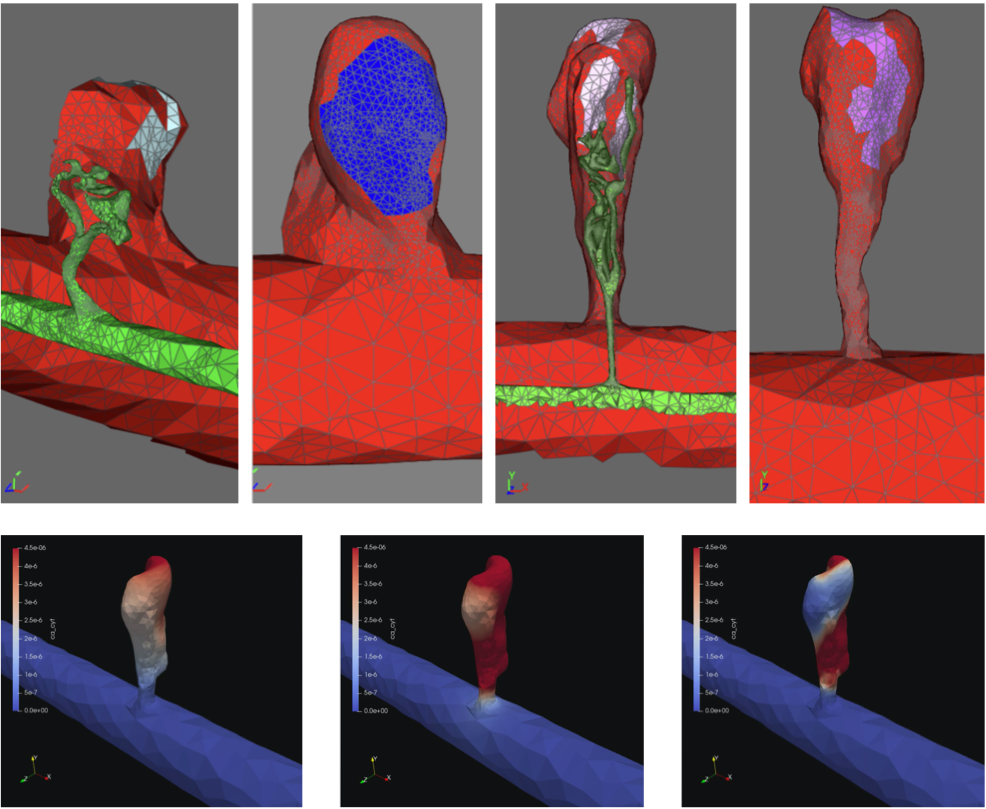
\includegraphics[scale=0.35]{inc/img/spine-types-simulation.png}
\caption{\textbf{Spine reconstructions and simulations:} (Top) Examples of spine reconstructions in collaboration with Dr. Vlachos (University of Freiburg, Germany). Reconstructions show variability in spine shape (red) as well as ER organization (green). (Bottom) Time sequence of a calcium simulation on reconstructed spine and dendrite geometry. Color scheme: red: max. calcium concentration, blue: min. calcium concentration}
\label{fig:spine-types}
\end{framed}
%\end{wrapfigure}
\end{figure}
\noindent\textbf{Numerical method:} To computationally solve the model problem, the triangular surfaces meshes of synaptic spines (see Fig.~\ref{fig:schematics} (C, D)), which have been generated from electron microscopy data (in collaboration with Dr. Vlachos, University of Freiburg, Germany) will be used to produce tetrahedral volume meshes using ProMesh (\cite{Reiter2012}). Using a first order finite volume method \cite{Eymard2000} the model equations are discretized on the previously generated surface and volume meshes. The nonlinear parts of the model, i.e. the Neumann boundary conditions are linearized with a Newton iteration. The resulting system of linear equations are solved by a geometric multigrid (GMG) method which is preconditioned using Bi-CGSTAB.  The GMG solve of the linear system uses 3 iterations of pre- and post- smoothing, both of which use the \textit{incomplete LU} factorization of the system matrix. We also set the \textit{SuperLU} library as the base solver for our large, sparse, nonsymmetric matrix problem. A backward Euler method is used to solve the problem in time. The proposed numerical methods are available in uG4, which will be used for all proposed computations. \\
%For numerical simulations, the four equations are
%discretized in space using a finite volumes method, \cite{Eymard2000}.
%%Control volumes are constructed as a Voronoi-like dual tesselation of the original
%%tetrahedral mesh by connecting the mid-points of edges, faces and volumes through planar facets.
%%The equations above must hold for all control volumes, giving rise to one equation per control volume.
%Time discretization is realized using a backwards Euler scheme. The described PDE problem
%should be solved by a multigrid method, \cite{Brandt1977,Fedorenko1962,Hackbusch1976,Ruge1987}. \\\\
%\textcolor{red}{Need to explain which parameters we want to vary etc.} \\\\
\noindent \textbf{Estimate of proposed simulation runs:}
Next we describe the simulations we will perform for the above project and anticipated resources. The accuracy of the simulations relies on the following: employing physiologically correct geometries, running the simulations on geometries processed through several levels of grid refinements, running the simulations with small time step size $\Delta t$ to capture the calcium dynamics in the cytosol and ER volume, and running the simulations with long end times. The studies we will perform are as follows:
\begin{itemize}
\item[1.] \texttt{Baseline runs} -- In order to study the physiological dynamics inside the dendrite we first run simulations without ER present to establish a baseline of calcium concentrations and general passive behavior of the calcium inside the dendrite geometry. We will run 10 simulations using a different calcium influx value with end time $t_f=0.02\ s$ and $\Delta t = 0.5\ \mu s$ which equates to $\frac{t_f}{\Delta t} = $ 40,000 time steps.
\item[2.] \texttt{RyR runs} -- Next we run simulations with active ER having ryanodine receptors (RyR) and SERCA pumps activated. For these simulations we run a parameter sweep on the density of RyR on the ER, this will establish the critical RyR density for calcium to be released from the ER into the cytosol. We sweep the RyR density value from 0 to 10 RyR per $\mu m^{2}$ at increments of 0.01, this amounts to 1,000 simulation runs. These simulations have an end time of 20 milliseconds since coupling of calcium in the dendritic region of the cell has been observed during the first 20 milliseconds of spine activation. This simulation set also has 40,000 time steps with $\Delta t = 0.5\ \mu s$.
\item[3.] \texttt{Calcium Pulse runs} -- Next we run studies for at least 3 seconds to observe the coupling effects between the spine region of the neuron and the dendrite region of the neuron for a fixed RyR density and different calcium influx pulse frequencies. These particular simulations will be performed with supercritical RyR density, each at 1 Hz, 3 Hz, 5 Hz, 10 Hz, and 20 Hz frequencies. This totals to 5 simulations, each with end time of 3 seconds, $\Delta t = 0.5\ \mu s$, this equates to $\frac{3.00}{0.5\times 10^{-6}}=$ 6,000,000 time steps.
\end{itemize}
We have 9 different spine-dendrite geometries that will undergo each of the above simulations. Currently, with the XSEDE trial account, we ran these simulations with 0 refinement (20,605 Degrees of Freedom -- DoFs) and 1 refinement (164,840 DoFs) on the Spine-Dendrite geometry and time step size $\Delta t =0.5\ \mu s$. In Fig.~\ref{fig:spine_dend_strongscaling} we show strong scaling for a geometry \textit{without ER}. We ran a simulation with 164,840 DoFs across 384 cpu cores which took 4.69 minutes = 0.0782 hours with simulation end time 0.02 seconds. Therefore the number of core hours = $384\ cores \times 0.0782\ hours =  30.02$ core-hours. In order to capture accurate results we will process geometries with at least 1 level of refinement, with and without ER geometry present. In Table \ref{tab:sus} we indicate the anticipated compute time requirements for the sub-projects. The total number of runs is determined by $(\#\text{runs} / \text{cell})\times(\#\text{cells})$; for instance, the \texttt{Baseline runs} are 10 simulations and there are 9 cell geometries, therefore, we have $(10\ \text{runs} / \text{cell})\times(9\ \text{cells}) = 90\ \text{runs}$. 
Then the number of core-hours are computed by $(\#\text{runs})\times(\text{core-hours}/ \text{run})$; therefore, for \texttt{Baseline runs} we have $(90 \ \text{runs})\times(30\ \text{core-hours}/\text{run}) = 2700$ core-hours. Similarly for the \texttt{RyR runs} we have $2700$ core-hours. For the \texttt{Calcium Pulse runs} we need to take into account the number of time steps since the end time is 3 seconds, we have $\frac{30\ \text{core-hours}}{40000\ \text{time-steps}}\times 6000000\ \text{time-steps} = 4500 $ core-hours.

Concerning storage requirements: we have two types of data output, text files in .txt format that contain the average calcium concentration in the volume and surface regions of the cell geometry and Visualization Toolkit files (vtk) for rendering and visualizing data in 3 dimensions. We will be generating .vtk output for the Calcium Pulse runs with active RyR \& SERCA pumps and we anticipate that each vtk file is 0.24 GiB at 1 refinement level. 

%\begin{figure}[H]
\begin{wrapfigure}[43]{r}{0.4\textwidth}
\centering
\begin{framed}\raggedleft%\centering
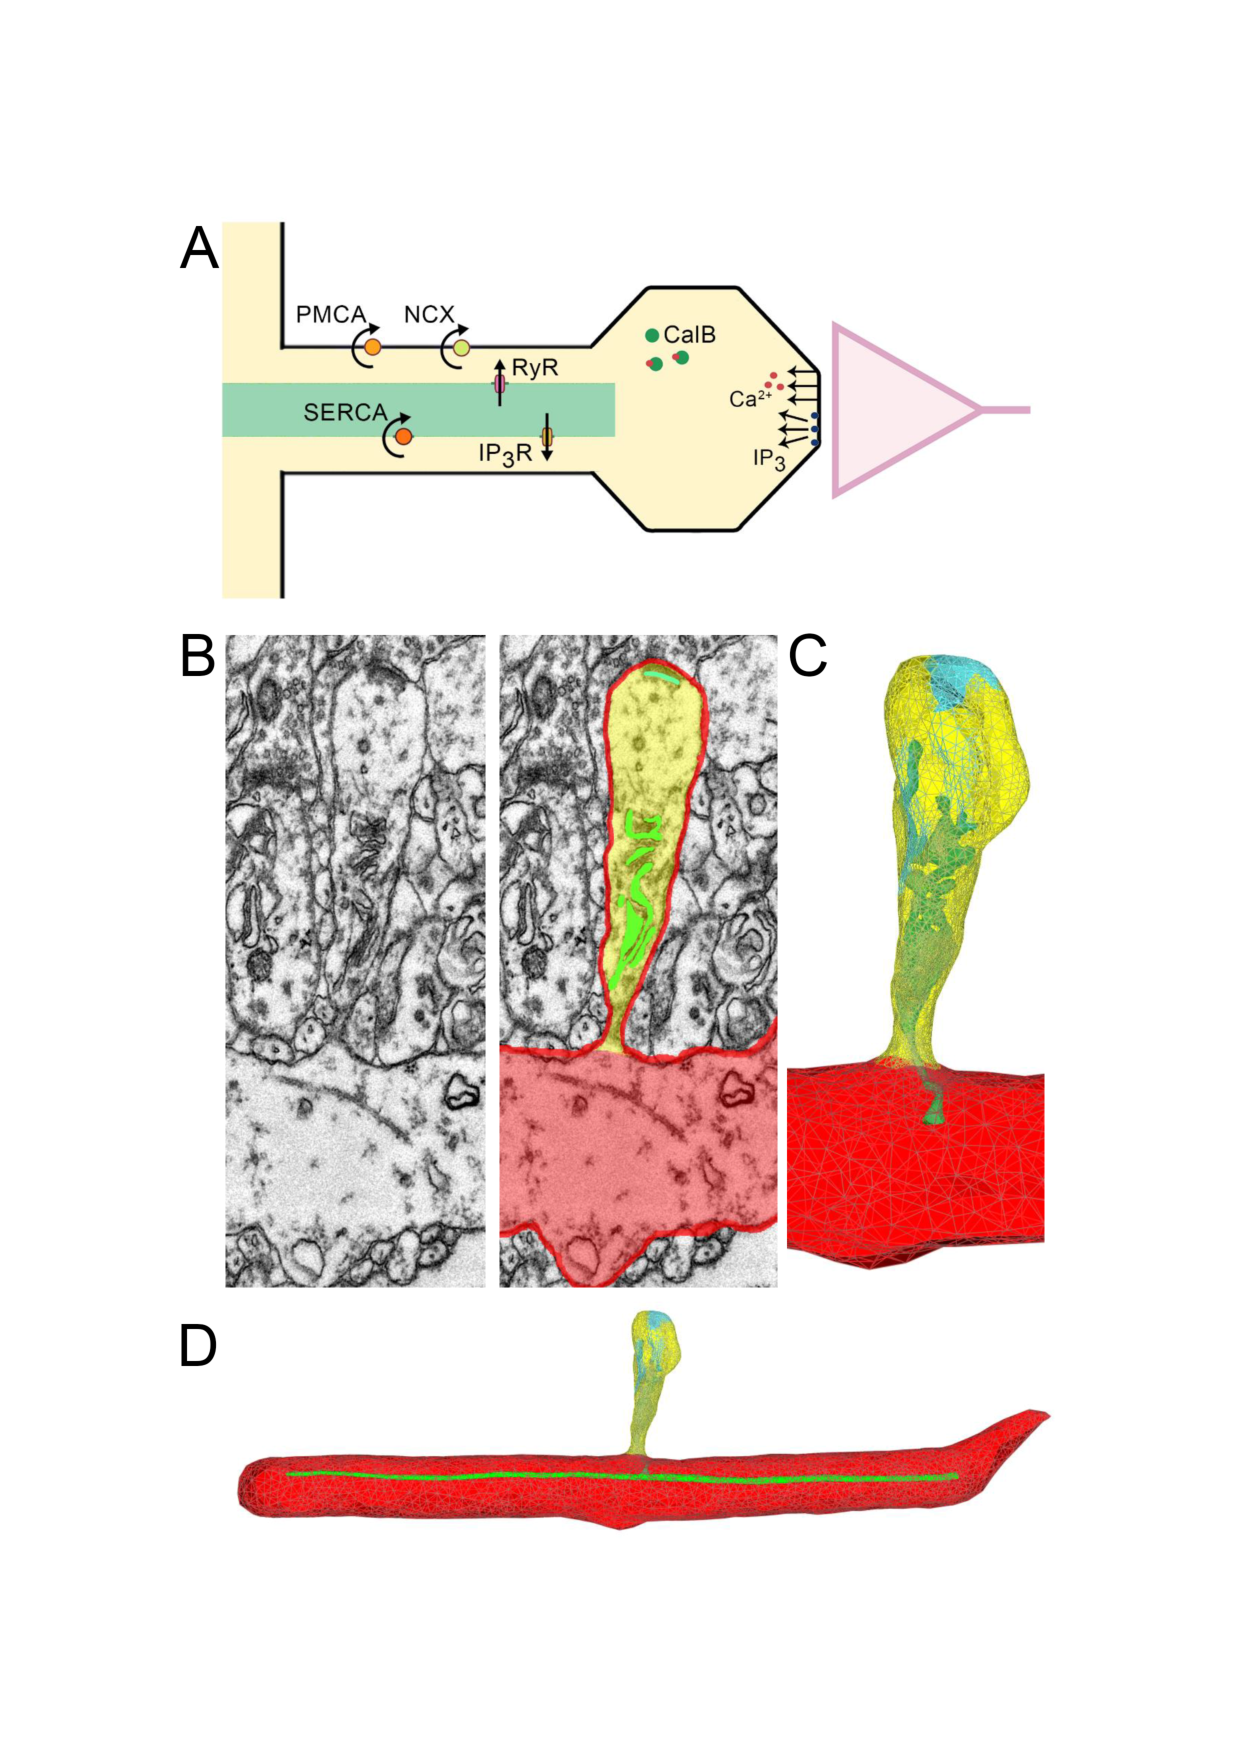
\includegraphics[scale=0.35]{inc/img/EM-spine.pdf}
\caption{\textbf{Calcium dynamics and spine reconstruction}: (A) Schematics of calcium model used in the proposed project. Calcium entry and IP3 production at the postsynaptic density induces a calcium signal in the cytosol (yellow) that propagates via a diffusion-reaction model towards the ER (green). Calcium exchange mechanisms on the plasma membrane (PMCA and NCX) and on the ER membrane (SERCA, IP3R, RyR) define nonlinear boundary conditions and drive calcium-induced calcium waves into and along the dendrite. (B) Example of electron microscopy image of a spine (left) and the marked regions of the morphology (right). (C) 3D reconstruction using (B). (D) reconstruction of a part of the dendrite and dendritic ER, connected to spine.} 
\label{fig:schematics}
\end{framed}
\end{wrapfigure}
%\end{figure}

The Calcium Pulse simulations run for 3 seconds and total 6 million time steps but we will require only 100 vtk time samples (equally distributed in time) out of the 6 million time steps. For the Calcium Pulse runs with active RyR \& SERCA pumps we will require $\left(0.24\frac{\text{GiB}}{\text{file}}\right)\times (100\ \text{files}) \times (9\ \text{cells})\times (5\ \text{freq.})=$ \textbf{1,080 GiB} of vtk storage for all nine cells and five frequencies. For the Calcium Baseline runs each simulation run will produce 2,750 kB (for end time of 0.02 seconds) of data in the form of text files, at 10 runs for 9 cells this equates to $\left(2750\frac{\text{kB}}{\text{run}}\right)\times (10\ \text{runs})\times (9\ \text{cells}) = $ 0.2475 GiB. For the RyR \& SERCA pump simulations we will be performing 1,000 simulation runs: $\left(2750\frac{\text{kB}}{\text{run}}\right)\times (1000\ \text{runs})\times (9\ \text{cells}) = $ 24.75 GiB. For the Calcium pulse simulations we have a run time 3 seconds which equates to 412,500 kB per run; therefore, $412,500\times 15\times 9 = $ 55.6875 GiB. Therefore, in total we anticipate \textbf{$0.2474+24.75+55.6875=$ 80.685 GiB} for text data; hence, for all spine simulations we anticipate $80.685 + 1,080 = $ 1.16 TiB. If we include ER geometry and dynamics this will incur more storage; therefore, we anticipate per month approximately \textbf{2 TiB} after which all data will be copied to local storage.
%150 runs.
%Approximately 50 shorter runs for development of the (parallel) correctness of the MPI program and to improve the parallel efficiency 
%of the novel DSMG method and to demonstrate the scaling behaviour of the method will be required. 
%Additionally the numerics of the newly developed DSMG algorithm needs to be compared to a standard
%numerical problem, a time-dependent convection-diffusion equation on a reconstructed
%neuron. To test for robustness of the numerical code 10 cells will be reconstructed,
%5 simulation setups (boundary conditions and initial conditions will be varied around a reference case) 
%will be run with the standard multigrid algorithm and 5 simulation setups will be run with the new
%DSMG algorithm. Results of the runs each will be compared concerning convergence and precision
%of the simulation result and contrasted with the results published in \cite{Breit2018}.
%\textcolor{red}{Old text:} \\
%In this sub-project the calcium dynamics in a compartmentalized neuron will be modeled.
%The endoplasmic reticulum (ER) is a multifunctional intracellular organelle of a neuron,
%which consists of a complex three-dimensional network of connected endomembrane
%tubules, stacks and cisternae, and is involved in various ion exchange processes,
%%cf. Fig.~\ref{fig:schematics},
%\cite{Breit2018}, ultimately responsible for synaptic plasticity, `cell within a cell'
%structure, cf. \cite{Berridge1998}.
%
%\begin{figure}
%\centering
%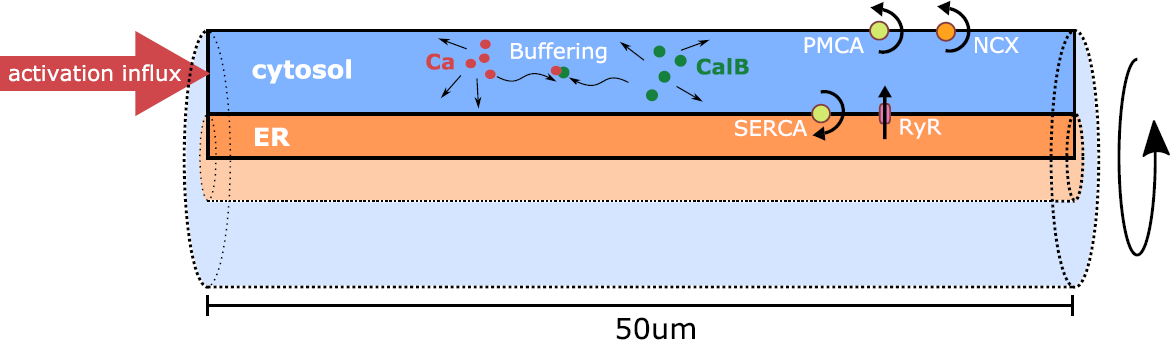
\includegraphics[scale=0.25]{inc/img/schematics.png}
%\caption{\textbf{Model geometry}. Simulation domain and model components. The example domain is a cylindrical dendrite 50 $\mu$m in length with variable radius containing a centrally positioned cylindrical ER of variable radius. The rotational symmetry of the domain was used to reduce the problem to two dimensions (axial and radial position). The calcium model contains calcium in the cytosol and the ER as well as calbindin (CalB) in the cytosol. The dynamics of both are governed by a diffusive process and a buffering reaction. Calcium can cross the ER membrane through RyR channels and SERCA pumps, the plasma membrane through PMCA and NCX pumps.}
%\label{fig:schematics}
%\end{figure}
%
%Of interest are the three-dimensional spatio-temporal $\textrm{Ca}^{2+}$ and $\textrm{IP}_3$ dynamics in the intracellular space of a neuron.
%This is modeled by a system of diffusion-reaction equations described in the following.
%The boundary conditions for this partial differential equation system are specifed by certain $\textrm{Ca}^{2+}$ and $\textrm{IP}_3$-dependent fluxes which depend on the chosen electrophysiogical stimulation protocol of the neuron.
%Mobility in the neuron respectively ER is described by diffusion equations for the four quantities calcium (cytosolic ($c_c$) and endoplasmic ($c_e$)), calbindin-D28k ($b$), and $\textrm{IP}_3$ ($p$), which is required to model $\textrm{IP}_3$ receptors embedded in the endoplasmic membrane
%\begin{equation}
%\frac{\partial u}{\partial t} = \nabla \cdot (D \nabla u)
%\end{equation}
%where $u(x, t)$ stands for the four quantities mentioned above.
%The diffusion constants $D$ are defined by data available in the literature \cite{Allbritton1992, Schmidt2003}.
%The interaction between cytosolic $\textrm{Ca}^{2+}$ calbindin-$\textrm{D}_{28k}$ (CalB) is described by:
%\begin{align}
%  \mathrm{Ca}^{2+}+\mathrm{CalB}\;\xrightleftharpoons
%  [\kappa_{b}^{-}]{\kappa_{b}^{+}}\;[\mathrm{CalBCa}^{2+}].
%\end{align}
%
%\noindent The full domain equations for cytosolic calcium and calbindin are thus given by
%\begin{align}
%  \delT{\ccyt} & \;=\; \nabla \cdot \left( D_{c} \nabla \ccyt \right) \;+\;
%    \left(\kappa_{b}^{-}\left(b^{\mathrm{tot}}-b\right)
%        -\kappa_{b}^{+}\:b\:\ccyt\right), \label{eq:ccyt}\\
%  \delT{b} & \;=\; \nabla \cdot \left( D_{b} \nabla b \right) \;+\;
%    \left(\kappa_{b}^{-}\left(b^{\mathrm{tot}}-b\right)
%        -\kappa_{b}^{+}\:b\:\ccyt\right)  \label{eq:buff}
%\end{align}
%
%\noindent Exponential IP\textsubscript{3} decay towards a basal IP\textsubscript{3} concentration
%$p^r$ in the cytosolic space is modeled by a reaction term that is added to the
%IP\textsubscript{3} diffusion equation, leading to the diffusion-reaction equation
%\begin{align}
%  \delT{\ip3} & \;=\; D_p\Delta\ip3 \;-\; \kappa_{\ip3}\left(\ip3-{\ip3}^{r}\right)
%\end{align}
%for IP\textsubscript{3} in the cytosolic domain.
%Endoplasmic Ca\textsuperscript{2+} dynamics are modeled by simple diffusion
%\begin{align}
%  \delT{\cer} & \;=\; D_{c}\Delta\cer
%\end{align}
%in the endoplasmic domain. For numerical simulations, the four equations are
%discretized in space using a finite volumes method, \cite{Eymard2000}.
%%Control volumes are constructed as a Voronoi-like dual tesselation of the original
%%tetrahedral mesh by connecting the mid-points of edges, faces and volumes through planar facets.
%%The equations above must hold for all control volumes, giving rise to one equation per control volume.
%Time discretization is realized using a backwards Euler scheme. The described PDE problem
%should be solved by a multigrid method, \cite{Brandt1977,Fedorenko1962,Hackbusch1976,Ruge1987}.
% If one designates with $\Omega_1$ the coarse domain and with $\Omega_2$ the fine
% domain and we require that the domains are nested, i. e. $\Omega_1 \subset \Omega_2$, and a restriction
%operator $\mathcal{R}$ and a prolongation operator $\mathcal{P}$ exist one
%can write the two grid iteration matrix by
%\begin{equation}
%u^{(i+1)} = G_2^{\nu_2}(Id - \mathcal{P}A_1^{-1}\mathcal{R}A_2)G_1^{\nu_1} u^{(i)} + \mathcal{P} A_1^{-1}\mathcal{R}f_2,
%\end{equation}
%where $Id$ is the identity matrix, $G_2$ a post smoothing matrix applied $\nu_2$ times, $G_1$ a pre smoothing matrix
%applied $\nu_1$ times, $A_1$ and $A_2$ the matrices arising from the discretized PDE problem on the coarse respectively
%fine domains $\Omega_1$ and $\Omega_2$ and $f_2$ the corresponding right hand side of the equation system arising by
%discretization on the coarse domain $A_2 u_2 = f_2$. 
%
%In traditional multigrid methods the restriction and prolongation operators are defined
%between the same space dimension, i.e. information transfer from a coarse to a fine
%grid level within the multigrid hierarchy. The \textbf{dimension-switching multigrid approach} 
%we are developing will involve a new multigrid base level of reduced dimensionality, 
%which will decrease computational cost. Some of the open topics are convergence rates and parallelization strategies.
%
%
%\noindent \textbf{Estimate of proposed simulation runs:} 150 runs.
%Approximately 50 shorter runs for development of the (parallel) correctness of the MPI program and to improve the parallel efficiency 
%of the novel DSMG method and to demonstrate the scaling behaviour of the method will be required. 
%Additionally the numerics of the newly developed DSMG algorithm needs to be compared to a standard
%numerical problem, a time-dependent convection-diffusion equation on a reconstructed
%neuron. To test for robustness of the numerical code 10 cells will be reconstructed,
%5 simulation setups (boundary conditions and initial conditions will be varied around a reference case) 
%will be run with the standard multigrid algorithm and 5 simulation setups will be run with the new
%DSMG algorithm. Results of the runs each will be compared concerning convergence and precision
%of the simulation result and contrasted with the results published in \cite{Breit2018}.
\subsection{Whole cell dynamics}\label{sec:whole-cell}
\textbf{The model:} While the first subproject in Sec.~\ref{sec:spine-model} focusses on the ultrastructure of individual synaptic spines, this subproject is defined on the whole cell level. This enables a rigorous analysis of how and when calcium signals are reliably relayed to the cell nucleus. The calcium model equations are the same as in Sec.~\ref{sec:spine-model}. The computational meshes are derived in the following way. The database NeuroMorpho.org (\cite{Ascoli2007}) hosts 1D geometry data of neurons. These data contain vertex and edge information of the neuron graph. Additionally each vertex stores the dendrite radius. With these input data, the tool AnaMorph (\cite{Moerschel2017}) will be used to generate surface meshes of the corresponding 1D geometry. The ER will be modeled as a neuron-within-neuron and can be generated alongside the surface reconstruction. In a final step the volumetric mesh is generated with ProMesh (\cite{Reiter2012}). The reconstruction pipeline is illustrated in Fig.~\ref{fig:anamorph}. Simulations will be run by initializing the calcium model with synapses. Synapses will be placed at distinct locations on the dendritic tree. Using standard synapse models calcium influx will be modeled as time-dependent Neumann boundary conditions. \\
\textbf{Expected outcome:} 
The ability for neurons to communicate calcium signals to the cell nucleus are critical for learning, plasticity, and cell survival (\cite{West2002, Milner1998, Bading2000, Hardingham1997}). 
In neuropathological situations, the calcium pathways are disrupted (\cite{Bezprozvanny2009, Chan2009, Cheung2008, Green2008}).
\begin{wrapfigure}[25]{r}{0.6\textwidth}
\vspace{-10pt}
\centering
\begin{framed}\raggedleft
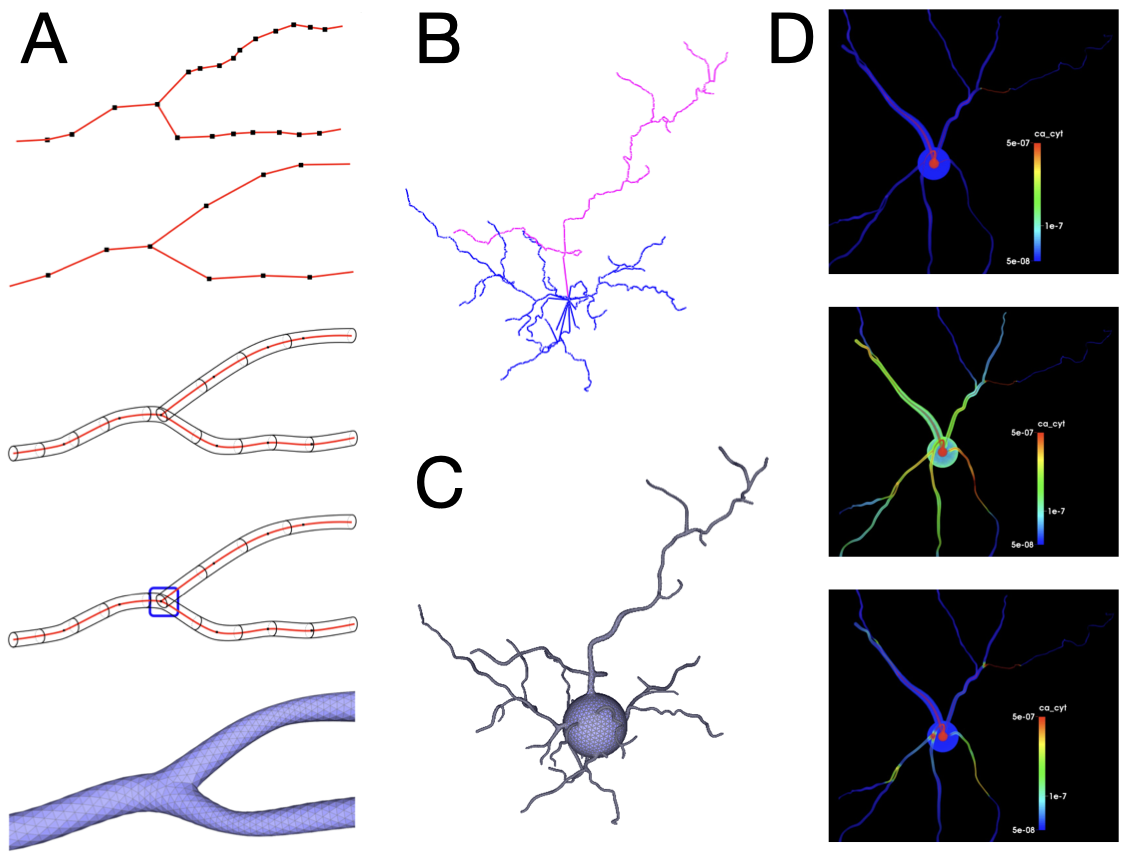
\includegraphics[scale=0.22]{inc/img/Anamorph.png}
\caption{\textbf{3D reconstruction pipeline}: (A) Illustration of cell surface reconstruction using graph and diameter information available from NeuroMorpho.org. The reconstruction pipeline begins with cellular graph information (B) and constructs a watertight surface triangulation (C), using the method presented in (\cite{Moerschel2017}). (D) Time evolution of a whole cell calcium simulation.}
\label{fig:anamorph}
\end{framed}
\end{wrapfigure}

We intend to study which conditions are necessary for neurons to reliably transmit calcium signals to the nucleus. We hypothesize that the spatio-temporal synaptic input patterns are relevant for synapse-to-nucleus communication. Thus, we intend to run simulations with different spatial synapse profiles and different temporal profiles, to test the influence of synapse clustering and synchronous vs. asynchronous activation. We further hypothesize that the morphological and biophysical parameters are important in stable communication. Thus, we plan to vary the dendrite to ER diameter ratios, as well as calcium channel and pump densities to determine threshold parameter sets that distinguish between stable and unstable synapse-to-nucleus communication. The results of this study could provide new insight into pharmacological intervention during e.g. synapse loss, which is a major contributor to Alzheimer's disease. \\
\textbf{Numerical method:} The numerical method for this sub-project is identical to Sec.~\ref{sec:spine-model}. \\
%We have been been developing simulation techniques
%for large-scale neuronal network simulations of networks described by graphs  (``1d'') with a
%diameter information attached to the vertices (representing idealized, cylindrical or
%cone-frustum compartments). The main results from this have been published in \cite{Breit2016}.
%We have also developed functionality to couple these large-scale 1d network simulations to fully
%resolved 3d reconstructed single-cell calcium simulations (similar to what is described in
%\cite{Grein14}). In this kind of simulation, we aim to understand the functional role of calcium
%as a messenger, taking into account the endoplasmic reticulum (ER) and a detailed model of the
%calcium dynamics including buffers as well as important endoplasmic and plasma membrane calcium
%exchange mechanisms such as the IP\textsubscript{3}R and RyR channels, voltage-dependent calcium
%channels, and sarco-/endoplasmic reticulum or plasma membrane calcium ATP-ases \cite{Breit13, Breit2018a, Breit2018b}.
%As the calcium dynamics are of special interest in the context of synaptic activity (e.g.,
%synapse-to-nucleus communication), examining a single fully resolved cell within an active
%network allows us to provide realistic synaptical inputs for the calcium simulation.
%But even with rather artificial inputs (as, e.g., given by an experimental stimulation protocol),
%single-cell calcium simulations and high-detail simulations of small regions of interest (as the
%vicinity of one or more dendritic spines) have become more and more important in our ongoing work.
%
%We would like to bring many aspects of the previous work together:
%The goal is to investigate whole-cell calcium dynamics on the basis of realistic synaptic input
%and membrane potential data from the 1d network model. In view of our basic parameter study
%about the influence of geometric parameters on calcium wave elicitation, we want to assess
%whether and under which circumstances calcium waves can occur within neurons in an active network:
%Which synaptic input patterns can lead to such waves? Can a single firing synapse cause a calcium
%signal cascade to the soma? Is the position of the synapse important (because of the
%location-specific geometry of the dendrites and ER)? Or are action potentials the only way to
%cause calcium influx into the soma (via voltage-dependent calcium channels)?
%What is the role of back-propagating action potentials? Do they significantly affect the local
%(synaptic) or even global calcium levels?
%Investigating these kinds of questions in simulations has been a long-standing goal of our
%research with implications for learning and cell survival. In past efforts a grid generation pipeline was developed with the
%goal in mind to reconstruct arbitrary cells from the \textit{Neuromorpho.org} database \cite{Ascoli2007}
%for the DMSG project and create a multigrid hiearchy. Existing tools, cf. \cite{Moerschel2017}, generated base levels too
%fine grained and thus not suitable for HPC solvers. A new ansatz was made by
%using spline data and grid generation tools from \ug which use point-diameter data.
%Volume meshes are generated efficiently by grid generation algorithms for constrained
%Delaunay triangulation \cite{Shewchuk2002, Si2005}. Based on these recent advances
%this sub-project aims to investigate by systematic parameter studies the calcium
%dynamics using the PNP model in the reconstructed cells on the sub-cellular level.
\noindent \textbf{Estimate of proposed simulation runs:} 
To study the cellular calcium dynamics from synapses to the cell nucleus, three computational setups will be used and solved on SDSC Comet. Representative computational meshes, which will be used in the
studies outlined below and used in the strong and weak scaling benchmarks have roughly 451,485 DoFs (see Tab. \ref{tab:speedup_whole_cell}, \ref{tab:speedup_whole_cell_strong}) with run times of roughly 5 minutes for 1,000 timestep on 3,074 processors.

\begin{enumerate}
\item \texttt{Variation of location of synaptic stimulation} -- We will use 10 neurons from the NeuroMorpho.org database and generate the 3D cell and ER geometries using the approach outlined above. Then we will vary the location of 500 synapses on the dendrites to determine the conditions under which calcium waves towards the nucleus are triggered. 

For these simulation setups a simulation time of $2$ seconds is necessary
to track calcium waves through the entire neuron. With a timestep $= 0.1$ ms this will amount to $10 \times \frac{2,000}{0.1} = 200,000$ timesteps for one specific synaptic stimulation pattern. To address the question how spatial variation of synaptic stimulation will affect calcium waves, 5 distribution patterns will be tested: homogeneously distributed synapses 1) close to soma, 2) on distal dendrites, 3) on proximal dendrites, and clustered synapses (non-homogeneous) 4) on distal dendrites, and 5) proximal dendrites. In total
$5 \times 10 \times \frac{2,000}{0.1} = 1,000,000$ timesteps will be necessary. Using the benchmark data above, this yields $\frac{1,000,000}{1,000} \times \frac{5}{60} \times 3072 = 256,000$ core hours.

\item \texttt{Variation of synaptic activation strength} -- Using the same 10 neurons we will vary synaptic strength to determine the conditions under which stable synapse-to-nucleus calcium communication is observed. 
For this study a simulation time of $2$ seconds is also necessary. We will test 3 settings: Low, intermediate and high synapse strength. Thus, in total we expect $3 \times 10 \times \frac{2,000}{0.1} = 600,000$ time steps, which yields $\frac{600,000}{1,000} \times \frac{5}{60} \times 3,072 = 153,600$ core hours.
\end{enumerate}
\begin{enumerate}[resume]
\item \texttt{Synapse loss study} -- We will employ 6 representative cells to study the effect of synapse loss on synapse-to-nucleus calcium communication. Comparing the healthy state (all synapses active) to pathological states in which we iteratively decrease the active synapse population by 10 \%, we will determine at which pathological states communication break-down is observed. 
Abortive calcium signals become visible in the first two seconds, thus we will set our end time to 2 s. Using a time step = $0.1$ ms to
resolve action potentials $20,000$ time steps are required for one neuron. In total, for 6 neurons with 10 states (1 healthy, 9 pathological) and 20,000 time steps for each simulation a total of $6 \times 10 \times \frac{2,000}{0.1} = 1,200,000$ time steps is required. Using the above benchmark data yields $\frac{1,200,000}{1,000} \times \frac{5}{60} \times 3,072 = 307,200$ core hours.
\end{enumerate}
For a summary of representative simulation runs, see Table \ref{tab:sus} with 
anticipated compute time (core-h / SUs) requirements for this sub-project. Storage requirement for one VTK file is roughly 1 $MiB$ per time step. This yields, for all three studies, a total of 2.8 $TiB$.  


\subsection{Summary}
The resources required for the two projects outlined in Sec.~\ref{sec:spine-model} and \ref{sec:whole-cell} are summarized in Tab. \ref{tab:sus}. The graduate student James Rosado will be conducting all runs related to Sec.~\ref{sec:spine-model} and Stephan Grein will be responsible for all runs for Sec.~\ref{sec:whole-cell}. The postdoc Qingguang Guan and PI Queisser will support and advise efforts in both projects. \\

All participants in the project will have access to a shared file in which an estimated demand for compute time for the following project month can be submitted. Stephan Grein will coordinate the internal distribution of compute time for the subsequent month by weighing the individual demand against milestone deadlines, demand for conference contributions, theses finalizations and other constraints. Thus, contingent overflow as well as monthly over-demand can be minimized.\\\\

%\begin{ganttchart}[vgrid, hgrid, bar/.style={fill=blue!50},
%                    y unit chart = 0.4cm, y unit title = 0.4cm, title height=1,
%                    bar height=0.4]{1}{12}
%  \scriptsize
%  \gantttitle{Project Month}{12} \\
%  \gantttitlelist{1,...,12}{1} \\
%  \ganttgroup{\textbf{Spine}}{1}{12} \\
%    \ganttbar[bar/.style={fill=red}]{\scriptsize \textcolor{red}{Update}}{1}{6}
%  \ganttgroup{\textbf{Whole cell}}{1}{12} \\
%    \ganttbar[bar/.style={fill=red}]{\scriptsize \textcolor{red}{Update}}{1}{6}
%\label{tab:runs}
%\end{ganttchart}
